\section{Argobots}
\label{sec:argobots}
Argobots \cite{argobots-paper, argobot} is a lightweight low-level threading framework, which offers a portable library interface and allows specialized runtime management to the user. The main aim of Argobots is to provide a mapping between high-level abstraction to low leve implementations \cite{argobots-paper}, as well as offering a lightweight layer of execution. To this aim, Argobots implements lightweight parallel work units, such as user-level threads (ULT) and tasklets, which are non-preemptable and offers, respectively, different models of execution. Work units are executed by OS-level threads, which in this context are referred to as Execution Streams (ESs). Each ES can be associated to a set of \textit{pools}, which are containers of work units, and execute tasks in the order provided by \textit{scheduler} entities. Argobots allows to define various scheduler (included custom ones), which determine the order of execution of each work unit inside the pools. Scheduler entities can be ``plugged'' at runtime to change the strategy of execution, based on requirements adapting to the computation at hand. Moreover, work units can be dinamically moved to a different pool in order to allow computation on a different ES.\newline

A generic Argobots application is depicted in \hyperref[fig:argobot-app]{\textbf{Figure \ref{fig:argobot-app}}}, which is built by following the execution flow shown in \hyperref[fig:ex-flow]{\textbf{Figure \ref{fig:ex-flow}}}. We can see how different pools can be associated to the same ES and how the scheduler provides the work units to the execution flow, which is sequential and guarantees progress. We describe in the next sections the characteristics of each building block of an Argobots application.

\begin{figure}[H]
    \centering
    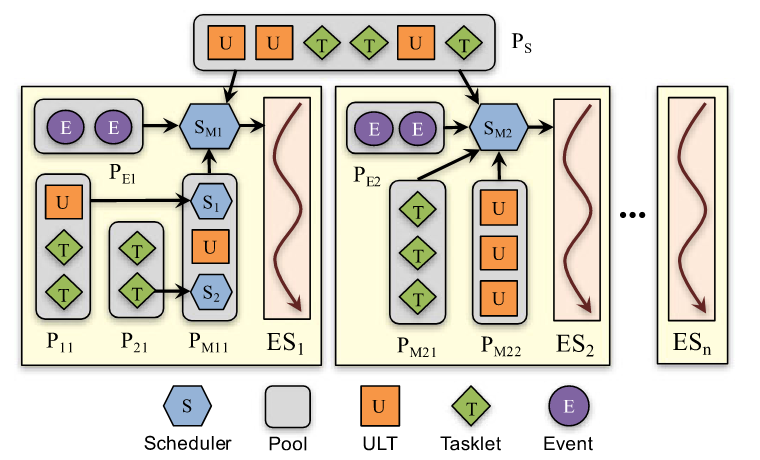
\includegraphics[width=0.8\linewidth]{res/argobot_application.png}
    \caption{Argobots execution model.}
    \label{fig:argobot-app}
\end{figure}

\begin{figure}[H]
    \centering
    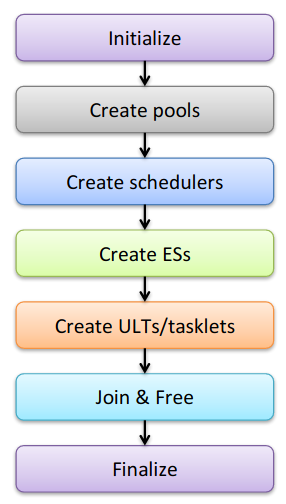
\includegraphics[width=0.35\linewidth]{res/control-flow.png}
    \caption{Argobots application flow of execution.}
    \label{fig:ex-flow}
\end{figure}

\subsection{Building blocks}
\subsubsection{Execution Streams}
Executions streams represents a sequential and independent instruction stream, which can consist of one or multiple non-preemptive work units (namely, ULTs and tasklets), it is mapped to a Pthread and can be bound to a hardware processing element such as CPU core or hardware thread. The work units to be executed are contained in one (or more) pools, and they are retrieved from one (or more) schedulers. Scheduling policies can be tweaked during runtime, and they determine the order in which work units flow to the execution stream and are thereby executed sequentially.\newline

Given the sequential nature of an ES, work units which are executed by the same ES do not require expensive synchronization mechanisms, since they do not run concurrently. However, synchronization is needed between work units executed in different ES running in parallel. 

\subsubsection{Schedulers}
Schedulers are responsible to deliver work units to the ES they are associated with, and they can implement different scheduling policies, which determines how work units are retrieved from pools and handled to the ES. Schedulers can be composed and scheduled just like work units, in order to compose different scheduling approaches dynamically, related to the computation at hand. Since a scheduler is considered as a work unit, it can be inserted into a pool and executed, which translates in a change of scheduling policy for the ES in charge, which will shift back to its original scheduler when the computation associated with the current scheduler is over.

\subsubsection{ULTs and Tasklets}
User-level threads and tasklets, also called \textit{work units}, represent two different types of workflow. User-level threads are independent execution units, which are executed in user space and can yield control to the scheduler, they can be dynamically migrated on a different execution stream during execution, since they have a private stack and context-saving capabilities. Tasklets, on the other hand, are considered to be ``lighter'' than ULTs, since they do not incur in costs related to context saving and stack management. They should be considered as atomic units of execution, which can't yield to a different execution and run to completion without context switching or suspension. 

\subsubsection{Pools}
Pools are containers of work units, and their sole purpose is to act as a uniform way of associating work to ES, indirectly, through schedulers. The only property associated with pools is the one regarding access, which can be set as private or shared. Shared pools may be used to implement a ``work-stealing'' strategy between two or more ESs. Pools are also used internally by the ES to receive asynchronous events.\newline

A pool associated with a running or stacked scheduler defines a set of work units ready to execute, which have to be controlled by the application programmer, since Argobots does not implicitly defines dependencies between work units. Hence, synchronization mechanisms offered by the library must be used to control the control flow of different work units.  Various operations can be performed over pools, like migration of work units to or from a specified pool, creation, destruction, and of course pop and push operations.

\subsection{Operations}
Argobots defines a set of operations which are common to all work units, made exception for some of them which are not available to Tasklets, given their execution model limitations. Implemented operations refer to:
\begin{itemize}
    \item Creation: allows the creation of work units, which are then inserted in a specific pool in a ready state. The type of pool and the associated scheduler(s) will determine the time and context of execution;
    \item Join: work units can be joined by other ULTs, which wait for their termination;
    \item Yield: a work unit can cooperatively yield control to the scheduler which is executing in the current ES at the time of yielding. The scheduler will then gather the next work unit to be executed following the implemented policy;
    \item Yield\_to: a ULT can decide to yield control to a specific ULT in the same ES. This operation avoids the overhead of one context switch by bypassing the scheduler;
    \item Migration: allows work units to be migrated between pools;
    \item Synchronization: ULT can rely over usual synchronization mechanisms implemented by Argobots, such as mutexes, condition variables etc.
\end{itemize}

\subsection{Memory Management}
Argobots is intended to be used in fine-grained dynamic environments, where creation and destruction of work units, as well as context switch between them, take place at high frequencies.\newline

Since, as shown in \cite{argobots-paper}, memory allocation and deallocation contribute to most of the time required to create and destroy a work unit, Argobots developed its own memory allocator. The memory allocator creates, for each ES, a memory pool which is subsequently used to manage all creation and destruction calls of work units. The memory pool is held private per ES, in order to avoid heap access synchronization upon creation of work units by means of the same ES. The size of the pool is tied to the number of work units which are spawned and allows to return memory to the system upon their destruction, if the pool reached a given threshold.\newline

Context switching, on the other hand, has a lower cost in terms of memory, compared to creation and destruction of work units, and it is only related to ULTs, since tasklets are atomic operations and can't yield to other work units. Context switching costs are mostly associated with:
\begin{itemize}
    \item ULT suspension: context of the currently running ULT must be saved and context of the next ULT must be resumed. However, the first step can be avoided if the yielding ULT is terminating and will not be resumed later;
    \item ULT join: the join operation suspends the caller and yield control to the scheduler, until the joined ULT terminates its execution. However, if two ULTs are in the same ES, the joining ULT can directly yield control to the joined ULT, bypassing the context switch to the scheduler entity.
\end{itemize}

% \subsection{Mixing Argobots with standard library threads}
% During the testing phase, we analyzed but still not tracked down an annoying drawback of mixing up two threading environments together. FastFlow uses standard library thread calls to run each node in a different thread, instead Argobots internally creates its own thread-mapped execution streams upon initialization, and associates a ``primary'' execution stream to the 